\documentclass[a4paper, 10pt, final]{article}
\usepackage{bonde}

\def\mytitle{Signal and Image Processing 2010}
\def\mysubtitle{Handin of mandatory excercise 3}
\def\myauthor{Ulrik Bonde}
\def\mymail{\mailto{bonde@diku.dk}}
\def\mydate{\today}

\title{\mytitle}
\subtitle{\mysubtitle}

\author{\myauthor{} - \mymail}
\date{\mydate}

\hypersetup{
colorlinks,%
citecolor=black,%
filecolor=black,%
linkcolor=black,%
urlcolor=black,%
bookmarksopen=false,
pdftitle={\mytitle{} - \mysubtitle},
pdfauthor={\myauthor}
}

\begin{document}
\maketitle

\subsection*{Question 3.1}
I have implemented a MATLAB program which creates ideal low- and
high-pass filters. Butterworth and High-frequency emphasis filtering are
also available, but only Butterworth filtering will be shown in the
following.

The filters work in the frequency domain which means that we first
Fourier transform the input image, then manipulate the transformed image
and finally do the inverse Fourier transform to see the result.

The filters use that the distance from the center of a shifted Fourier
transformed image corresponds to a frequency with low frequencies in the
center. Since MATLAB will complain if the results have negative values,
we use the absolute value of the results, thus eliminating values below
zero.

The ideal low-pass filter is defined as
\begin{equation}
    h(u, v) = \left\{ \begin{array}{l l l}
        1 & \mbox{if} & D(u, v) < D_0\\
        0 & \mbox{otherwise} &
    \end{array}\right.
\end{equation}
where we use $D(u, v) = \sqrt{ (u - \frac{M}{2})^2 + (v - \frac{N}{2})^2 }$
which is the distance from the center. The high-pass filter is the
inverse. The actual filter and it's effect on the image
\emph{square.tiff} is shown in fig. \ref{ideal}. The filters applied to
the image \emph{unix.tiff} is shown in fig. \ref{ideal_unix}. Inspect
the figures for further description on the filters.

To avoid the ringing effect, we now apply a smoother filter. The
Butterworth filter is defined as
\begin{equation}
    h(u, v) = \frac{1}{1 + \left[ D(u, v)/D_0 \right]^{2n}}
\end{equation}
We use $D(u, v)$ as defined above and $n = 2$.

The Butterworth filter have been applied to the image \emph{unix.tiff}
and the results are shown in fig. \ref{butter_unix}. Notice the shape of
the filter. The circle fades out allowing some high frequencies in the
final image by creating a smooth transition. Further description is
found the image caption.

\begin{figure}[!h]
    \centering
    \subfloat[Original]{\label{org_1}
\includegraphics[angle=0,width=0.35\textwidth]{images/square}}\hspace{1em}
    \subfloat[Fourier
    transform]{\label{ft_1}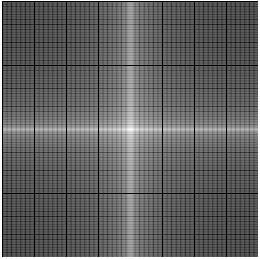
\includegraphics[angle=0,width=0.35\textwidth]{images/square_f}}\\
    \subfloat[Low-pass
    filter]{\label{low}
\includegraphics[angle=0,width=0.3\textwidth]{images/low_filter_35}}\hspace{1em}
    \subfloat[Modified Fourier
    transform]{\label{low_f}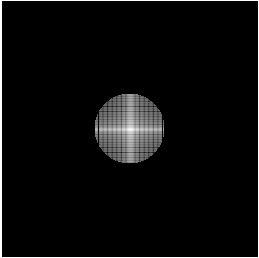
\includegraphics[angle=0,width=0.3\textwidth]{images/filter_f_square_low}\hspace{1em}}
    \subfloat[Resulting
    image]{\label{res_low}
\includegraphics[angle=0,width=0.3\textwidth]{images/square_low_result}}\\
    \subfloat[High-pass
    filter]{\label{high}
\includegraphics[angle=0,width=0.3\textwidth]{images/high_filter_35}}\hspace{1em}
    \subfloat[Modified Fourier
    transform]{\label{high_f}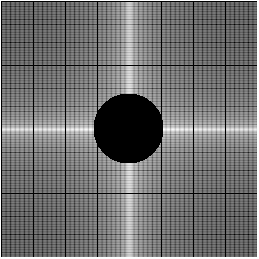
\includegraphics[angle=0,width=0.3\textwidth]{images/filter_f_square_high}\hspace{1em}}
    \subfloat[Resulting image]{\label{res_high}
\includegraphics[angle=0,width=0.3\textwidth]{images/square_high_result}}
    \caption[]{\textbf{Top row:} The original image and its
    corresponding Fourier transform. \textbf{Middle row:} The ideal
    low-pass filter, the filter applied in the Fourier domain and the
    resulting image. \textbf{Bottom row:} Same as above, but with a
    high-pass filter. Notice the ringing effect from the ideal filters.
    Both filters have $D_0 = 35$. The filters applied in the Fourier
    domain is the result of pointwise multiplication of the filter and
    the Fourier transformed image. Only pixels/frequencies with a value greater than
    zero in the filter will be expressed in the result.}
    \label{ideal}
\end{figure}

\begin{figure}[!h]
    \centering
    \subfloat[Original]{\label{orgideal}
\includegraphics[angle=0,width=0.3\textwidth]{images/unix}}\\
    \subfloat[$D_0 = 5$]{\label{low5}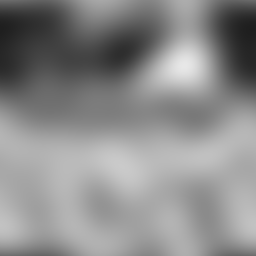
\includegraphics[angle=0,width=0.3\textwidth]{images/unix_low_result_5}}\hspace{1em}
    \subfloat[$D_0 = 15$]{\label{low15}
\includegraphics[angle=0,width=0.3\textwidth]{images/unix_low_result_15}\hspace{1em}}
    \subfloat[$D_0 = 45$]{\label{low45}
\includegraphics[angle=0,width=0.3\textwidth]{images/unix_low_result_45}}\\
    \subfloat[$D_0 =
    5$]{\label{high5}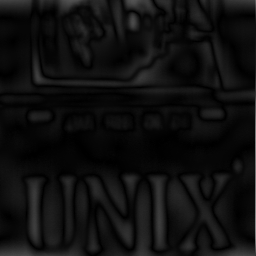
\includegraphics[angle=0,width=0.3\textwidth]{images/unix_high_result_5}}\hspace{1em}
    \subfloat[$D_0 =
    15$]{\label{high15}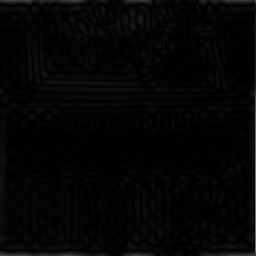
\includegraphics[angle=0,width=0.3\textwidth]{images/unix_high_result_15}\hspace{1em}}
    \subfloat[$D_0 =
    45$]{\label{high45}
\includegraphics[angle=0,width=0.3\textwidth]{images/unix_high_result_45}}\\
    \caption[]{Ideal filters applied. \textbf{Middle row:} Low-pass
    filtering.  Note that at lower cutoff-values the image is blurred.
    \textbf{Bottom row:} High-pass filtering. Even at low cutoff-values,
    a lot of information is lost. The take-away
    point is that the low frequencies hold much image information. This
    is shown by the fact that even with a low $D_0$ in high-pass
    filtering, much image information is lost. Note the ringing effect
    from the ideal filters.
    }
    \label{ideal_unix}
\end{figure}

\begin{figure}[!h]
    \centering
    \subfloat[Original]{\label{orgbutter}
\includegraphics[angle=0,width=0.3\textwidth]{images/unix}}\\
    \subfloat[$D_0 =
    5$]{\label{butter5}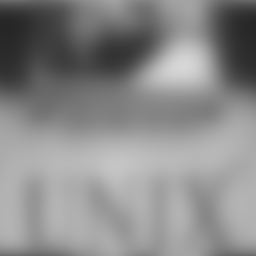
\includegraphics[angle=0,width=0.3\textwidth]{images/unix_butter_result_5}}\hspace{1em}
    \subfloat[$D_0 =
    15$]{\label{butter15}
\includegraphics[angle=0,width=0.3\textwidth]{images/unix_butter_result_15}\hspace{1em}}
    \subfloat[$D_0 =
    45$]{\label{butter45}
\includegraphics[angle=0,width=0.3\textwidth]{images/unix_butter_result_45}}\\
    \subfloat[$D_0 =
    5$]{\label{butterf5}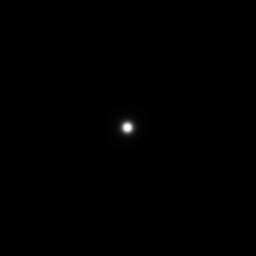
\includegraphics[angle=0,width=0.3\textwidth]{images/butter_low_filter_5}}\hspace{1em}
    \subfloat[$D_0 =
    15$]{\label{butterf15}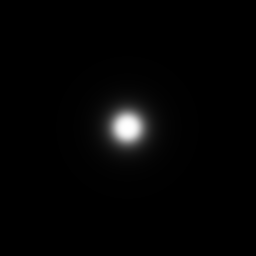
\includegraphics[angle=0,width=0.3\textwidth]{images/butter_low_filter_15}\hspace{1em}}
    \subfloat[$D_0 =
    45$]{\label{butterf45}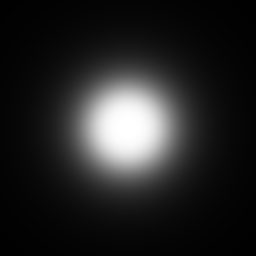
\includegraphics[angle=0,width=0.3\textwidth]{images/butter_low_filter_45}}\\
    \caption[]{Butterworth filters applied. \textbf{Middle row:} The
    resulting images. Again we notice that at low cutoff-values the
    image is blurred.
    \textbf{Bottom row:} The actual filters. Note that these filters do
    not cause the ringing effect. Also, the filter preserves the image
    information better. At $D_0 = 5$ the letters ``UNIX'' are more
    visible than the result using an ideal filter. At $D_0 = 45$ the
    image is almost the same as the original but with a slightly higher
    contrast.}
    \label{butter_unix}
\end{figure}

\clearpage

\subsection*{Question 3.2}
We let $M = 2^m$ and $N = 2^n$ and let $I$ be a $M \times M$ image and
$f$ a seperable $N \times N$ filter. In the following we assume that
$M \geq N$.

The naive convolution $(f \star I)(x)$, disregarding that $f$ is separable,
will yield $M^2N^2$ multiplications, as we for every pixel in $I$ will
have to multiply that with every pixel in the filter. This is infeasible
for large values of $N$ (remember that $M \geq N$).

Using that $f$ is separable we can split the filter and convolute the
rows and columns of $I$ separably. The image has $M$ rows. For each row
in $I$ we have $M$ pixels. The filter have been reduced to a 1D filter
of length $N$. Then for each pixel in a row we perform $N$
multiplications. The same is true for the columns in $I$, i.e.  $M$
columns with $M$ pixels which must be multiplied $N$ times. The total
amount of calculations needed for convolution in the spatial domain
$C_S$ is derived below.
\begin{align}
    C_S & = M(MN) + M(MN)\\
    & = 2M^2N
\end{align}

Now we want to find the number of multiplications needed in the
frequency domain. To do this we must Fourier transform both $I$ and
$f$, but we should also make sure that the size of $f$ is equal to the
size of $I$ (to do pointwise multiplication in the frequency domain). We
pad $f$ with zeroes to match the size of $I$.

The Fourier transform is separable and again we can transform a single
row (or column) with $L\log(L)$ multiplications. The image have $M$ rows
and each row require $M\log(M)$ multiplications. The same is true for
the columns. The filter require the same amount. We then get a total of
$2(2(M^2\log(M)))$ multiplications just for the Fourier transform of $I$
and $f$. We assume that the inverse Fourier transform use the same
amount of calculations, we also need $2(M^2\log(M))$ for transforming
$I$ back to the spatial domain. The actual convolution in the frequency
domain is just pointwise multiplication of $\mathcal{F}(I)$ and
$\mathcal{F}(f)$. This is $M^2$ multiplications. The total amount of
multiplications in the frequency domain is then:
\begin{align}
    C_{\mathcal{F}} & = 2(2(M^2\log(M))) + M^2 + 2(M^2\log(M))\\
    & = 6M^2\log(M) + M^2
\end{align}
It should be noted that the multiplications in the frequency domain are
complex multiplications.

When should we use convolution in the frequency domain rather than in
the spatial domain? This depends on the size of the filter. We solve the
inequality $C_{\mathcal{F}} < C_S$.
\begin{align}
    C_{\mathcal{F}} & < C_S\\
    6M^2\log(M) + M^2 & < 2M^2N\\
    3\log(M) + \frac{1}{2} & < N
\end{align}
When the filter size $N$ is greater than $3\log(M) + 1/2$ then fewer
multiplication will have to be done if we transform to the Fourier
domain and do the convolution there.

If $\mathcal{F}(f)$ is already known, we can cut away the
multiplications for the transform of $f$, thus only requiring
$4M^2\log(M) + M^2$ multiplications. For convolution in the frequency
domain to be feasible we then only require that $N > 2\log(M) + 1/2$.

Table \ref{table_sizes} shows when convolution in the spatial domain is
feasible and when to switch to the frequency domain.
\begin{table}[!h]
    \centering
    \begin{tabular}{|c|c|}
        \hline
        $M$ & Max $N$\\\hline
        $4$ & $4$ \\
        $8$ & $8$\\
        $16$ & $8$\\
        $32$ & $8$\\
        $64$ & $16$\\
        $128$ & $16$\\
        $256$ & $16$\\
        $512$ & $16$\\
        $1024$ & $16$\\
        $2048$ & $32$\\
        $4096$ & $32$\\
        \hline
    \end{tabular}
    \caption{Maximal filter size ($N \times N$) in
    an $M \times M$ image for feasible convolution in
    the spatial domain. If the filter is larger for a given $M$, less
    multiplications would be used in the frequency domain. For
    $M \geq 2048$ the max size for $N$ remains constant.}
    \label{table_sizes}
\end{table}

\subsection*{Question 3.3}
Two images have been handed out which have been corrupted by some
systematic interference and some random noise.

We first inspect the image \emph{noisy.tiff} shown in fig.
\ref{orgnoisy}. By inspecting the Fourier transform of the image (fig.
\ref{noisyfft}) we find the frequencies of the systematic pattern. They
can be seen as two ``stars'' in the diagonal. We would like to remove
these frequencies such that the interference do not show in the image.
For this we construct a very simple filter shown in fig.
\ref{noisymask}.

The result, where just the systematic interference have been removed can
be seen in fig. \ref{noisyinter}, but the image is still very noisy. We
apply a low-pass filter using a Butterworth filter with $D_0 = 65$ which
produce a pretty good result.

Other techniques have been tried to remove the remaining noise, such as
a median filter, but the low-pass filter yields the best visual result.

\begin{figure}[!h]
    \centering
    \subfloat[Original]{\label{orgnoisy}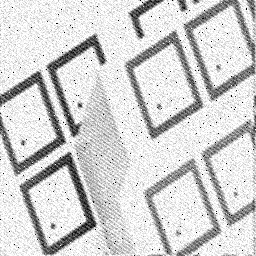
\includegraphics[angle=0,width=0.3\textwidth]{images/noisy}}\hspace{1em}
    \subfloat[Fourier transform]{\label{noisyfft}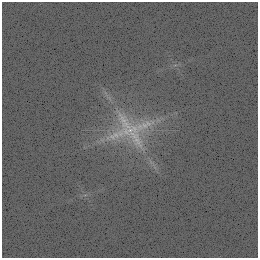
\includegraphics[angle=0,width=0.3\textwidth]{images/noisy_fft}}\hspace{1em}
    \subfloat[Mask]{\label{noisymask}\fbox{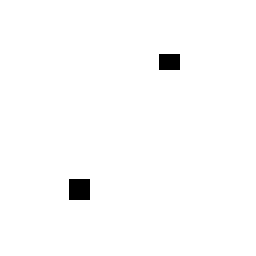
\includegraphics[angle=0,width=0.3\textwidth]{images/noisy_mask}}}\\
    \subfloat[Removed systematic interference pattern.]{\label{noisyinter}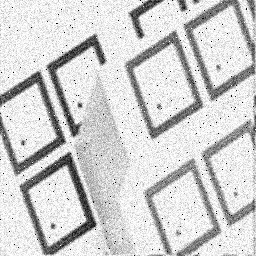
\includegraphics[angle=0,width=0.3\textwidth]{images/noisy_inter}}\hspace{1em}
    \subfloat[Butterworth filtering with $D_0 = 65$.]{\label{noisefinal}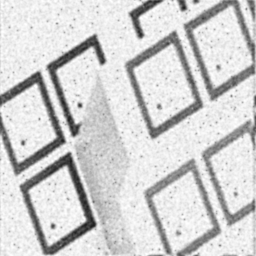
\includegraphics[angle=0,width=0.3\textwidth]{images/noisy_final}}
    \caption[]{
    Repair of the image \emph{noisy.tiff}.
    }
    \label{noisy}
\end{figure}

The second image is shown in fig. \ref{orgberlinger}. It's Fourier
transform in fig. \ref{berlingerfft} hints that two systematic
interference patterns corrupting the image (as we have two sets of
``stars''). Removing the large stars, those furthest from the center of
highest frequency, make no real difference in the image, but removing
those closest to the center removes the systematic interference (see
fig. \ref{berlingerinter}). While the systematic noise have been removed
the image is still noisy. Much like the previous image we use the
Butterworth filter to even out the noise. This lowers the contrast and
we also need to adjust the colors of the image. The final image in fig.
\ref{berlingerfinal} is a bit blurry, but much better than the original
image.

\begin{figure}[!h]
    \centering
    \subfloat[Original]{\label{orgberlinger}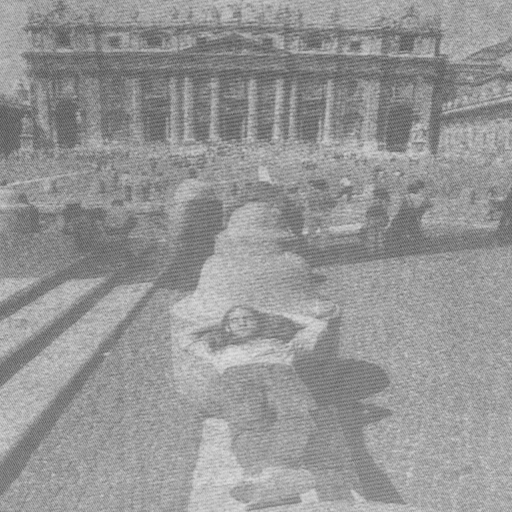
\includegraphics[angle=0,width=0.3\textwidth]{images/berlinger}}\hspace{1em}
    \subfloat[Fourier
    transform]{\label{berlingerfft}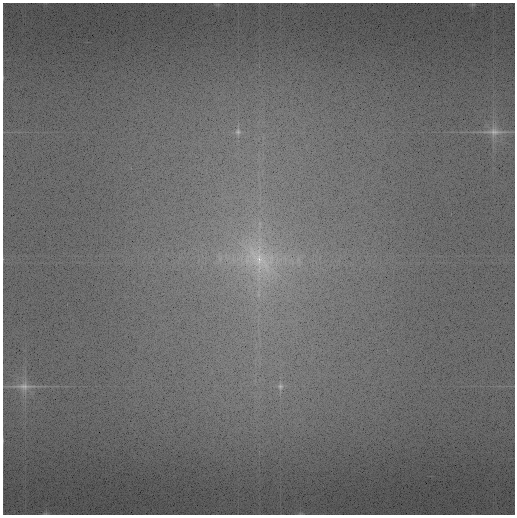
\includegraphics[angle=0,width=0.3\textwidth]{images/berlinger_fft}}\hspace{1em}
    \subfloat[Mask]{\label{berlingermask}\fbox{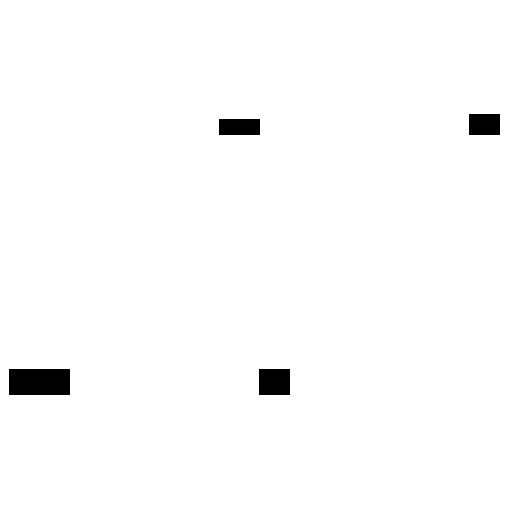
\includegraphics[angle=0,width=0.3\textwidth]{images/berlinger_mask}}}\\
    \subfloat[Removed systematic interference
    pattern.]{\label{berlingerinter}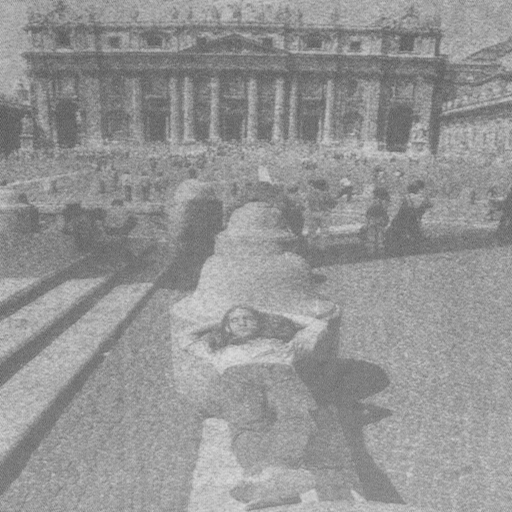
\includegraphics[angle=0,width=0.3\textwidth]{images/berlinger_inter}}\hspace{1em}
    \subfloat[Butterworth filtering with $D_0 =
    100$ and color adjustment.]{\label{berlingerfinal}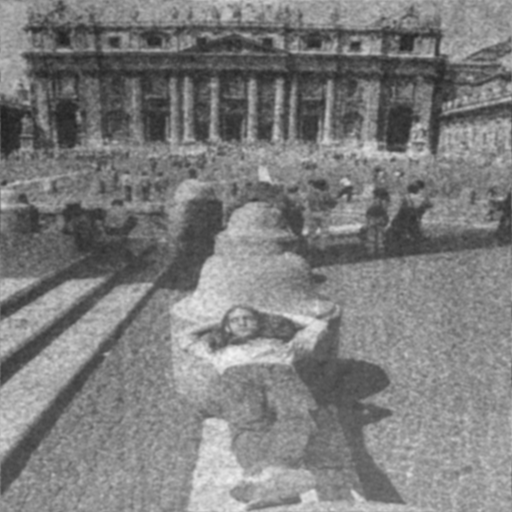
\includegraphics[angle=0,width=0.3\textwidth]{images/berlinger_final}}
    \caption[]{
    Repair of the image \emph{berlinger.tiff}.
    }
    \label{berlinger}
\end{figure}

%%%%%%%%%%%%%%%%%%%%%%%%%%%%%%%%%%%%%%%%%%%%%%%%%%%%%%%%%%%%%%%%%%%%
% Formal stuff

%\bibliographystyle{abbrvnat}
%\bibliography{bibliography}
%\addcontentsline{toc}{chapter}{Litteratur}

\end{document}

% vim: set tw=72 spell spelllang=en:
